\documentclass[preprint]{aastex}
\usepackage{natbib}
\usepackage{color}
\bibliographystyle{apj}
\usepackage{verbatim}

\begin{document}

\title{Mesogranulation in the Sun}
\author{Laurel Farris}
\affil{New Mexico State University}
\email{laurel@laurelfarris.com}

\begin{abstract}
    Evidence for structure on the mesogranular scale is investigated
    in the solar corona using data from the narrow 193\AA{} bandpass
    images taken with the Atmospheric Imaging Assembly (AIA) on board
    the Solar Dynamics Observatory (SDO). Cross-correlations centered
    on bright points in quiet sun regions and coronal holes were run
    for an hour-long limb-subtracted data cube.
\end{abstract}

\section{Introduction}\label{intro}
Evidence of intermediate structure on the photosphere between
granulation and supergranulation was first discovered by
\cite{November}, who coined the term ``mesogranules'' after detecting
vertical flows at scales between 5000 and 10000 km, lasting roughly
two hours. The driving mechanism behind the production of this
structure was still uncertain. There is a possible connection between
the horizontal size scales of granular structures at the photosphere
and the depth at which ionization occurs for H and He.
%(\cite{}).
Mesogranulation could be the ``missing scale'' connected to the second
ionization of He. It could also simply be an indicator of
``higher spatial harmonics of the primary supergranule cell''.

Further investigation of this elusive feature has been carried out
over the years$\ldots$

\section{Data}
\subsection{SDO and AIA}
AIA produces 12-second cadence images
in ten different passbands, each of which correspond
to a different height above the photosphere,
and most of which are different ionization states of Fe.
(\cite{Lemen}).
These levels of ionization and strongly dependent on temperature,
so AIA samples the ``full thermal range of the corona''. (source?)
The FeXII/XXIV line at 193\AA{} was used for this project,
at the ``corona and hot flare plasma'' region.
This particular line was sampled because $\ldots$?
Fe lines are the best emitters at high temperatures, and are much
cleaner then those of other elements, which can have more lines in a
given passband (source?).

\subsection{Data Aquisition}
The data was downloaded using \texttt{vsoget.pro} (cite Sam here?)

Since the focus of the project was general structure
over the solar surface, a relatively ``quiet''
(i.e.\ low magnetic activity)
data set was chosen.
An hour of data at full cadence was downloaded.
(include day/time data was taken).

\subsection{Data Reduction}
First, the limb was subtracted from the data cube,
which reduced the original images from
4096$\times$4096 to 2001$\times$2001 square pixels.
This new data cube was then aligned to subtract artificial variation
between images. An image of the full limb-subtracted disk is shown in
figure \ref{limb_sub} (with values raised to a power of 0.1 for better
visualization of the structures).


A few active regions are visible, as well as
some quiet sun areas in the upper right and a coronal hole in the
upper left.

\subsection{Data Analysis}
For simplicity, a few bright points (magnetic BPs? Or just ``bright
spots''?) were chosen from the region of the data where the
coronal hole is located.
% A closeup image of this region is shown in figure \ref{}.

A pixel located roughly in the center of each bright point
was cross-correlated with
every other pixel out to a radius of 50 pixels, or roughly 17500 km.
This extends well beyond the proposed maximum diameter of mesogranules
at 10,000 km. (commas in big numbers?)

\section{Results}

\begin{figure}
        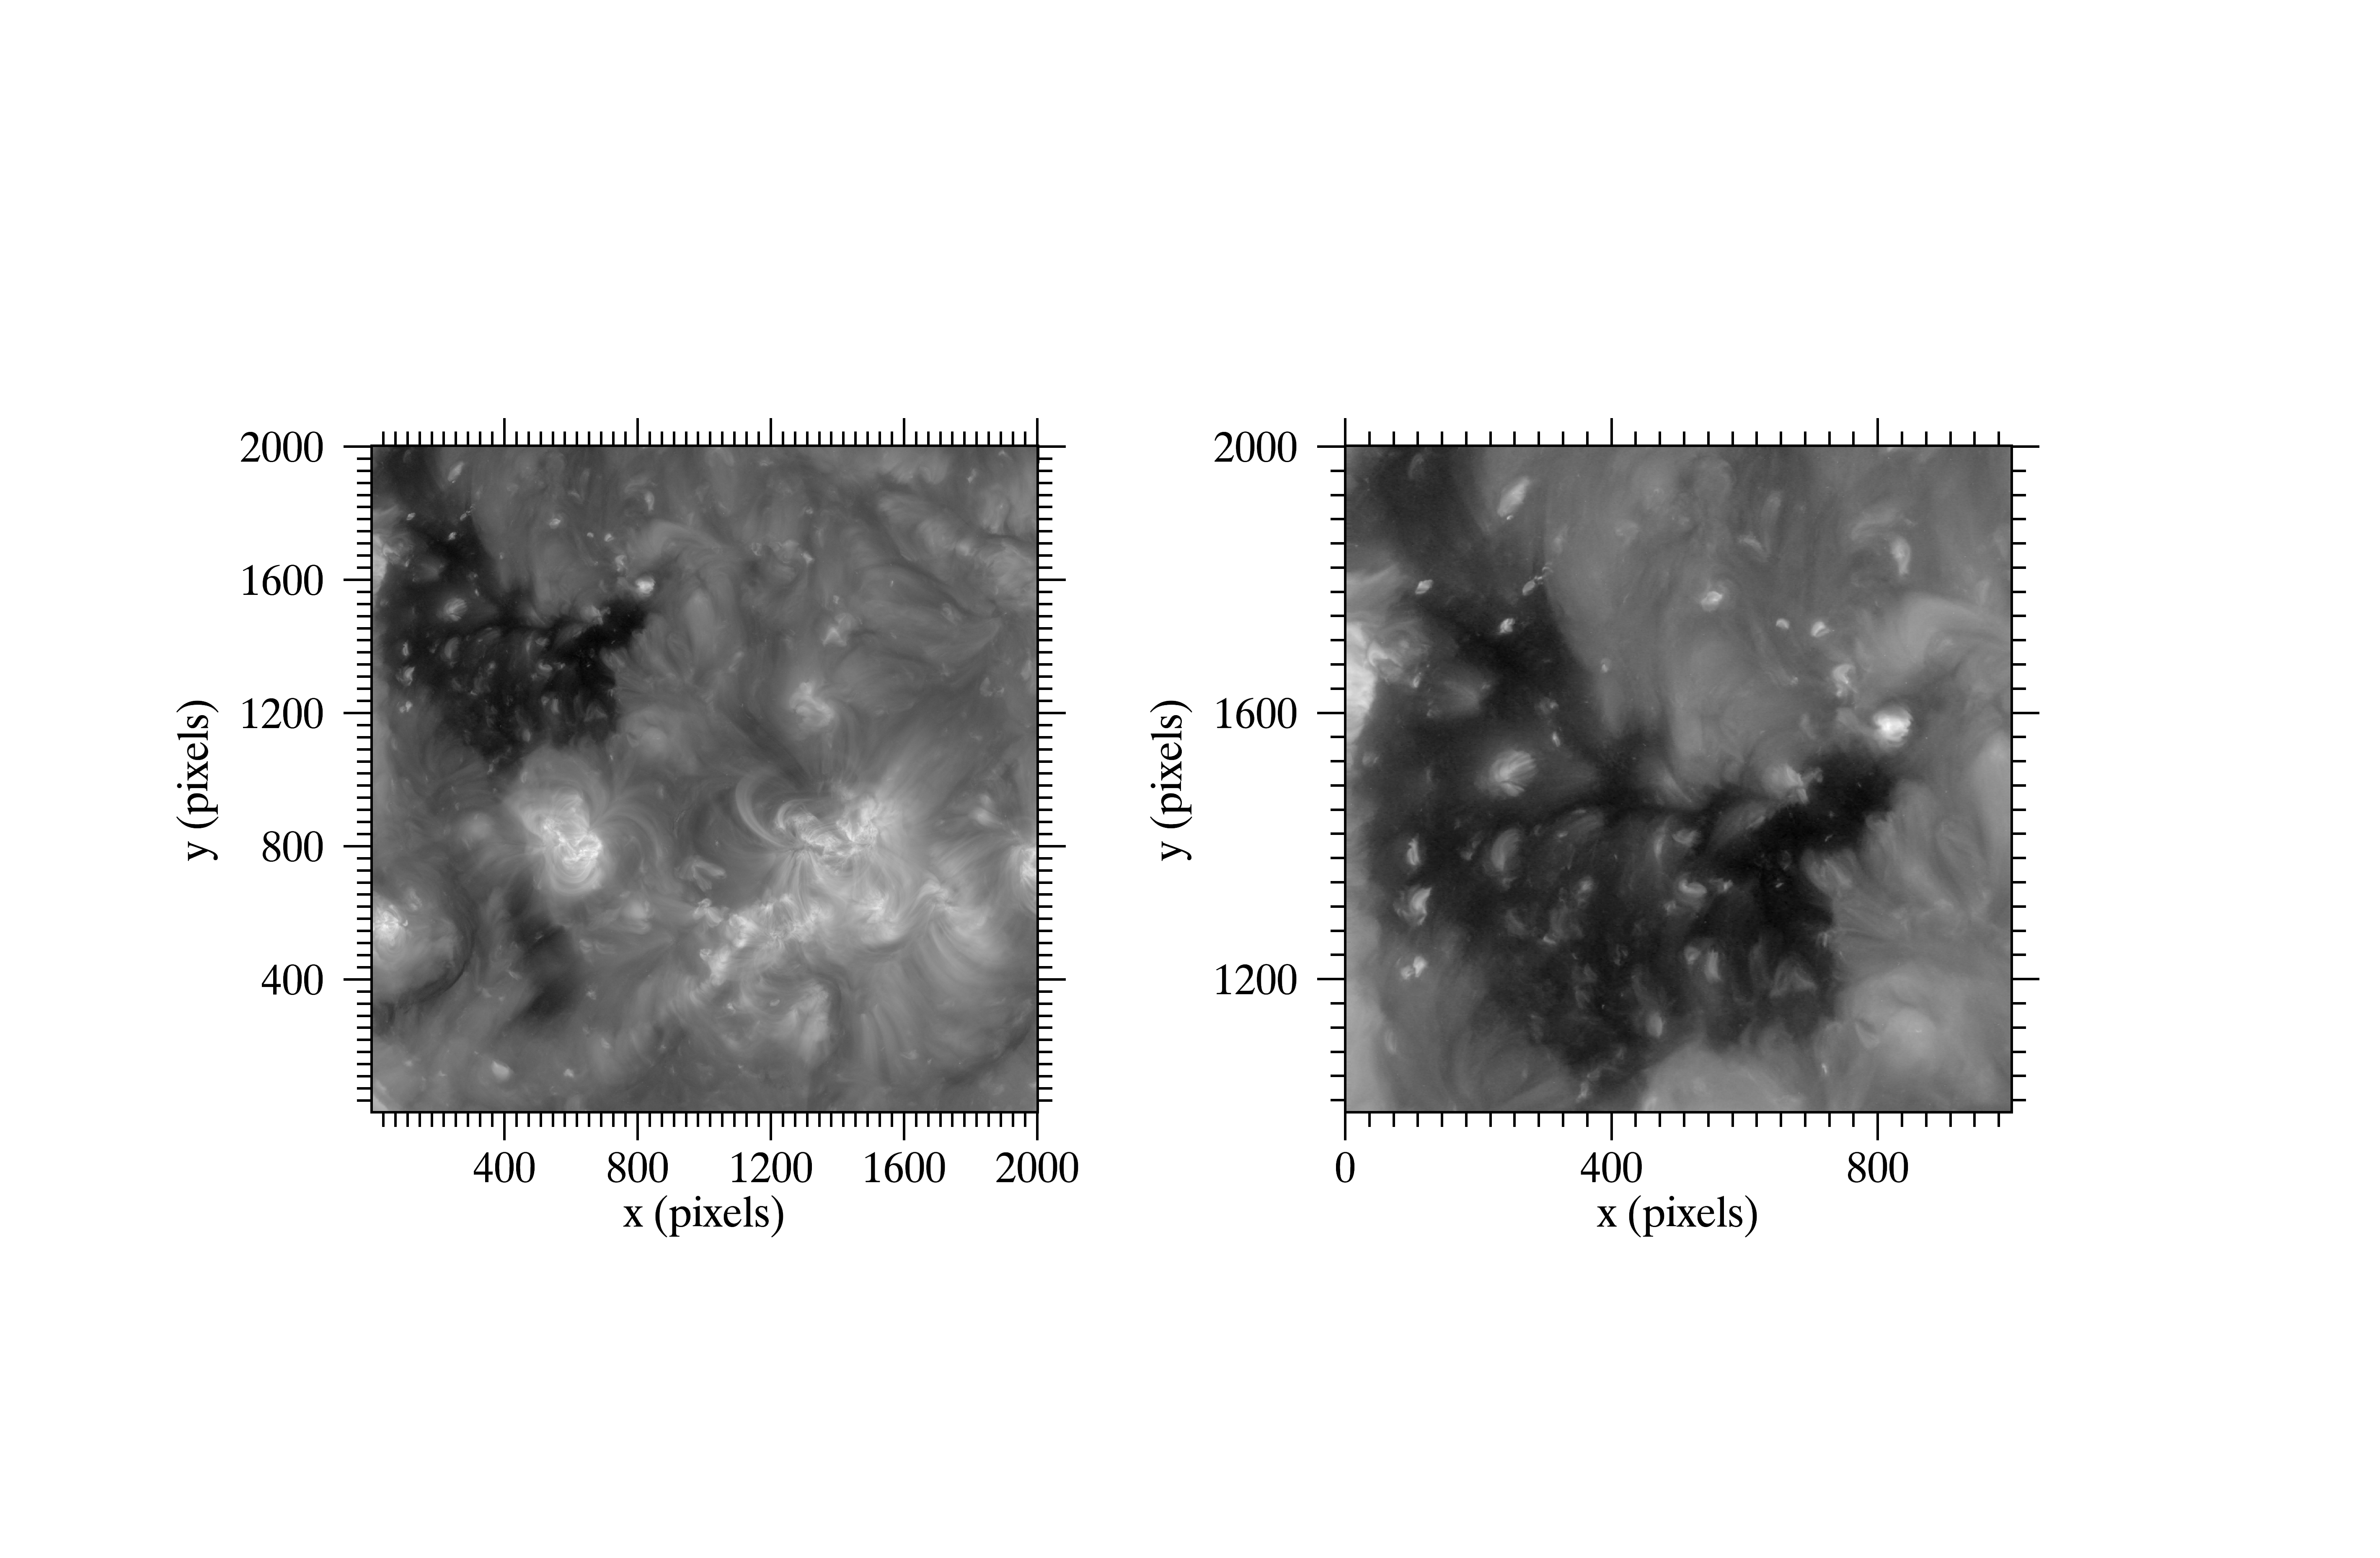
\includegraphics[width=\textwidth]{../figures/full_ch.png}
        \caption{Limb-subtracted disk and coronal hole (seen in
        upper left corner of full disk).}
\end{figure}%-------------------------------------------------------
\begin{figure}[htb!]
    \centering
    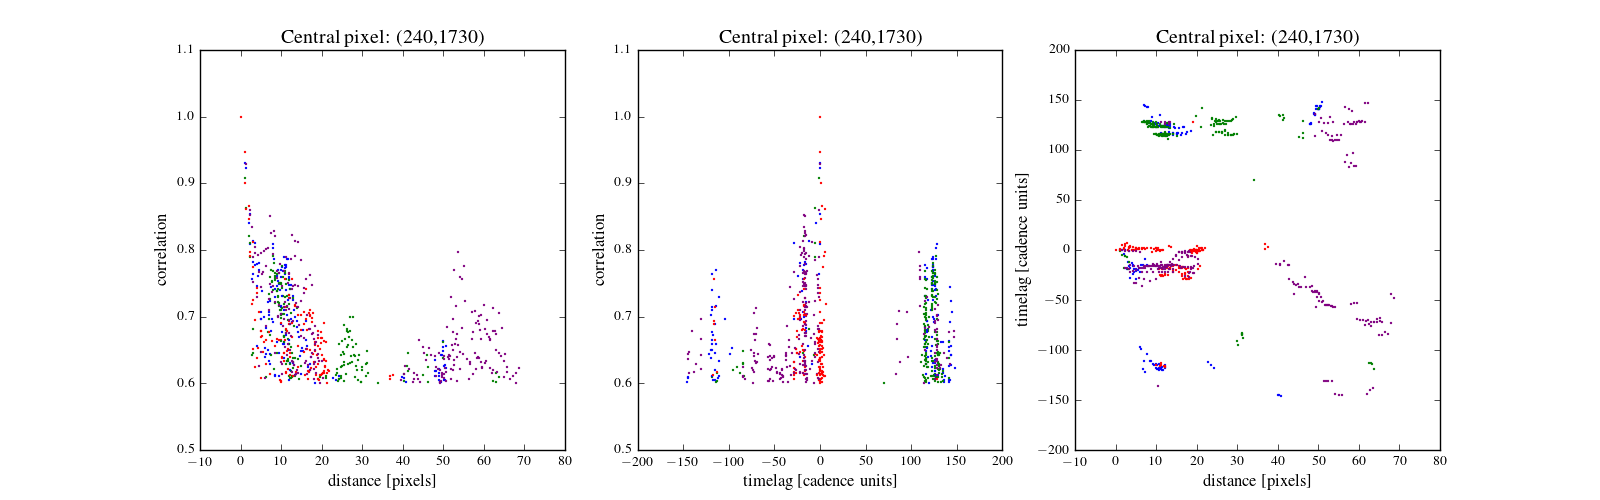
\includegraphics[width=\textwidth]{../figures/bp1_cool.png}
    \caption{Correlation as a function of distance for four bright
    points from the coronal hole}
\end{figure}
\begin{figure}[htb!]
    \centering
    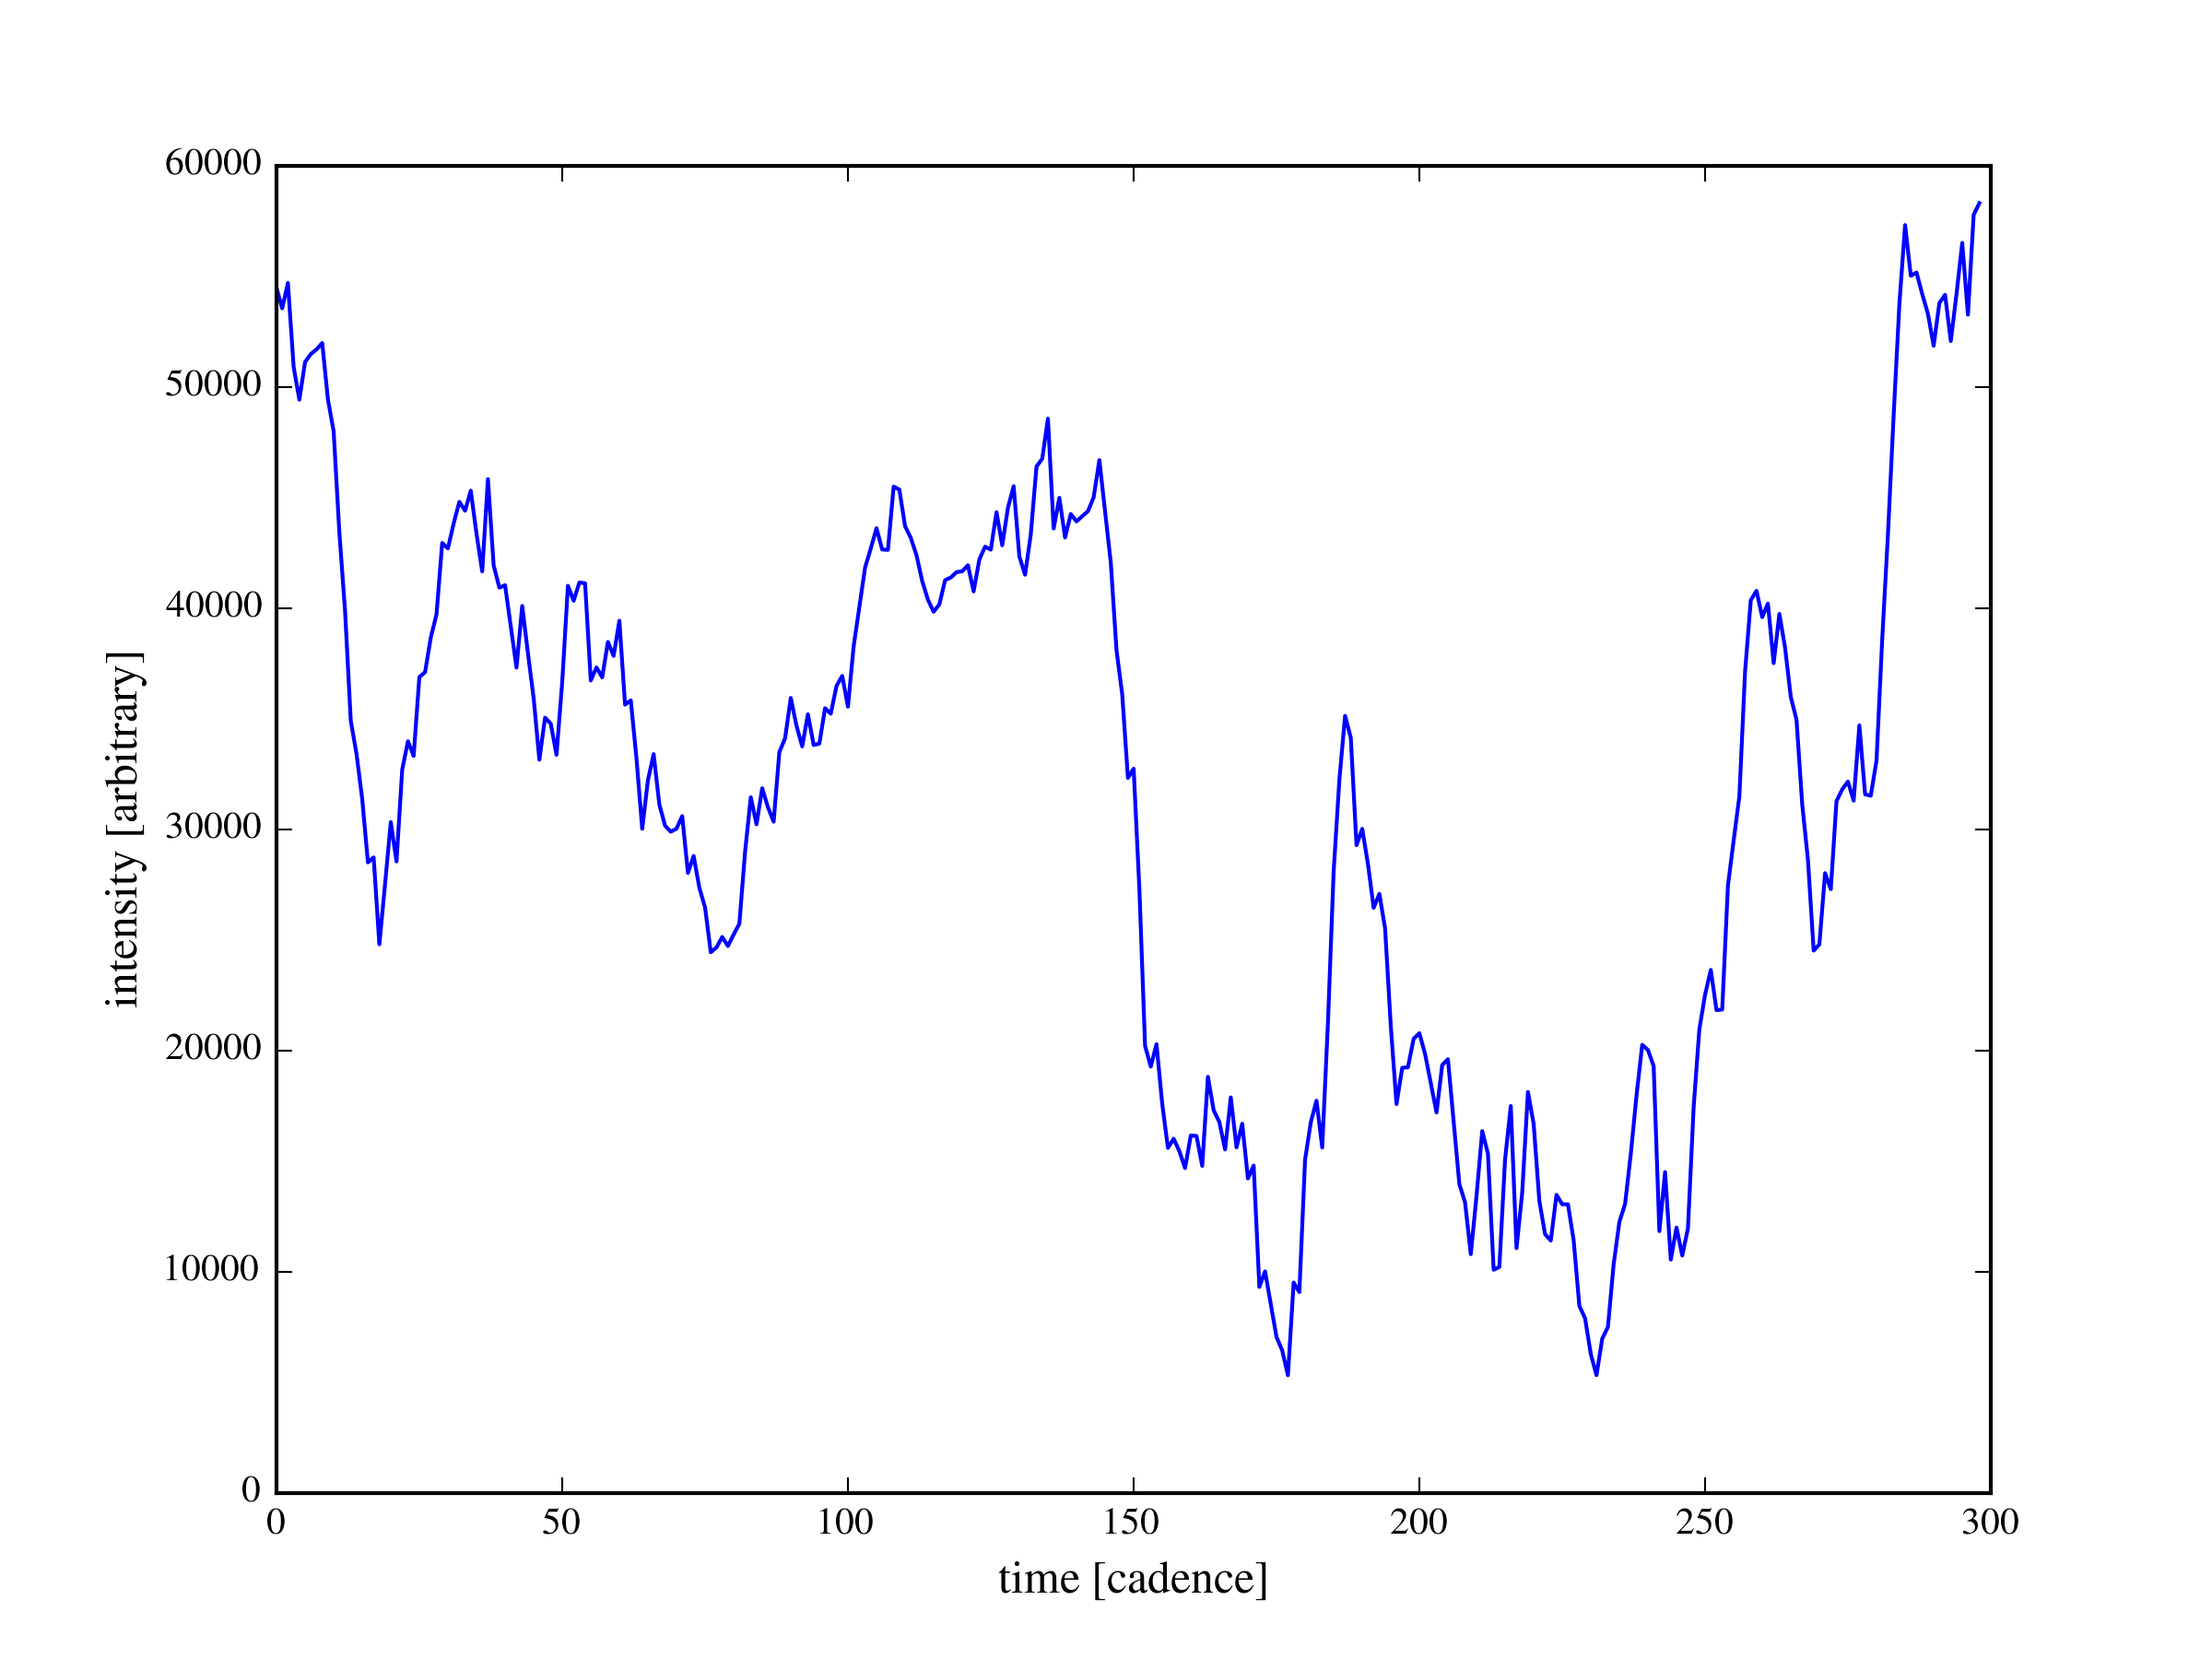
\includegraphics[width=\textwidth]{../figures/lightcurve2.png}
    \caption{lightcurve for one bright point - determined by
        intensity threshold of 100. There were 441 pixels summed up in
        every image in the data cube (?).}
\end{figure}
\begin{figure}[htb!]
    \begin{minipage}[b]{0.45\linewidth}
        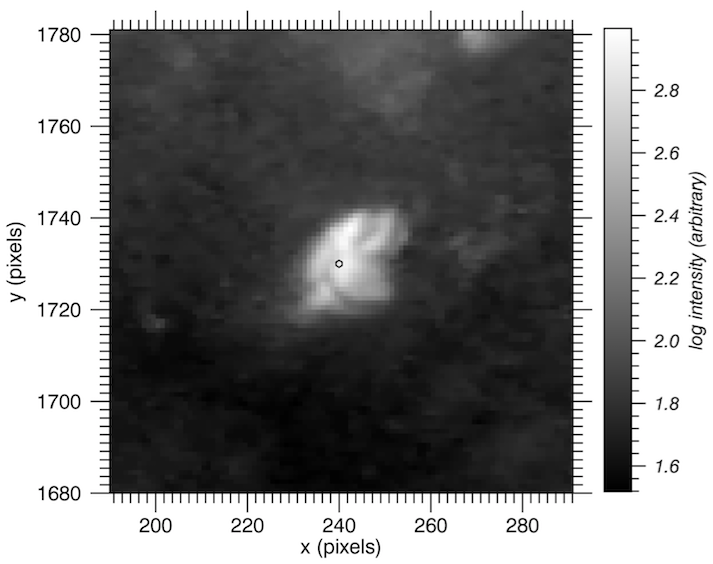
\includegraphics[width=\textwidth]{../figures/bp1_image.png}
        \caption{First bright point at (240,1730), which occupies an
        area of about 50 million km$^2$ (at this height).}
    \end{minipage}
    \quad
    \begin{minipage}[b]{0.45\linewidth}
        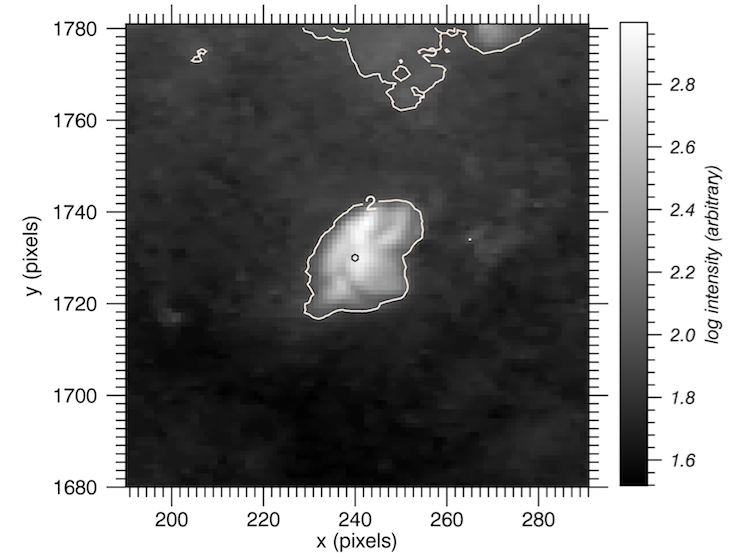
\includegraphics[width=\textwidth]{../figures/bp1_contour.png}
        \caption{Contour around intensity threshold.}
    \end{minipage}
\end{figure}

\begin{figure}[htb!]
    \centering
        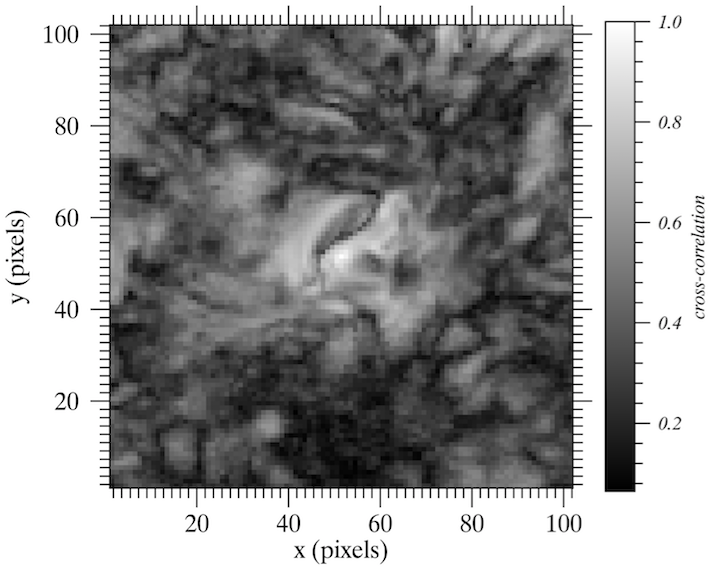
\includegraphics[width=\textwidth]{../figures/bp1_cc.png}
        \caption{Cross-correlation image}
\end{figure}
\begin{figure}[htb!]
        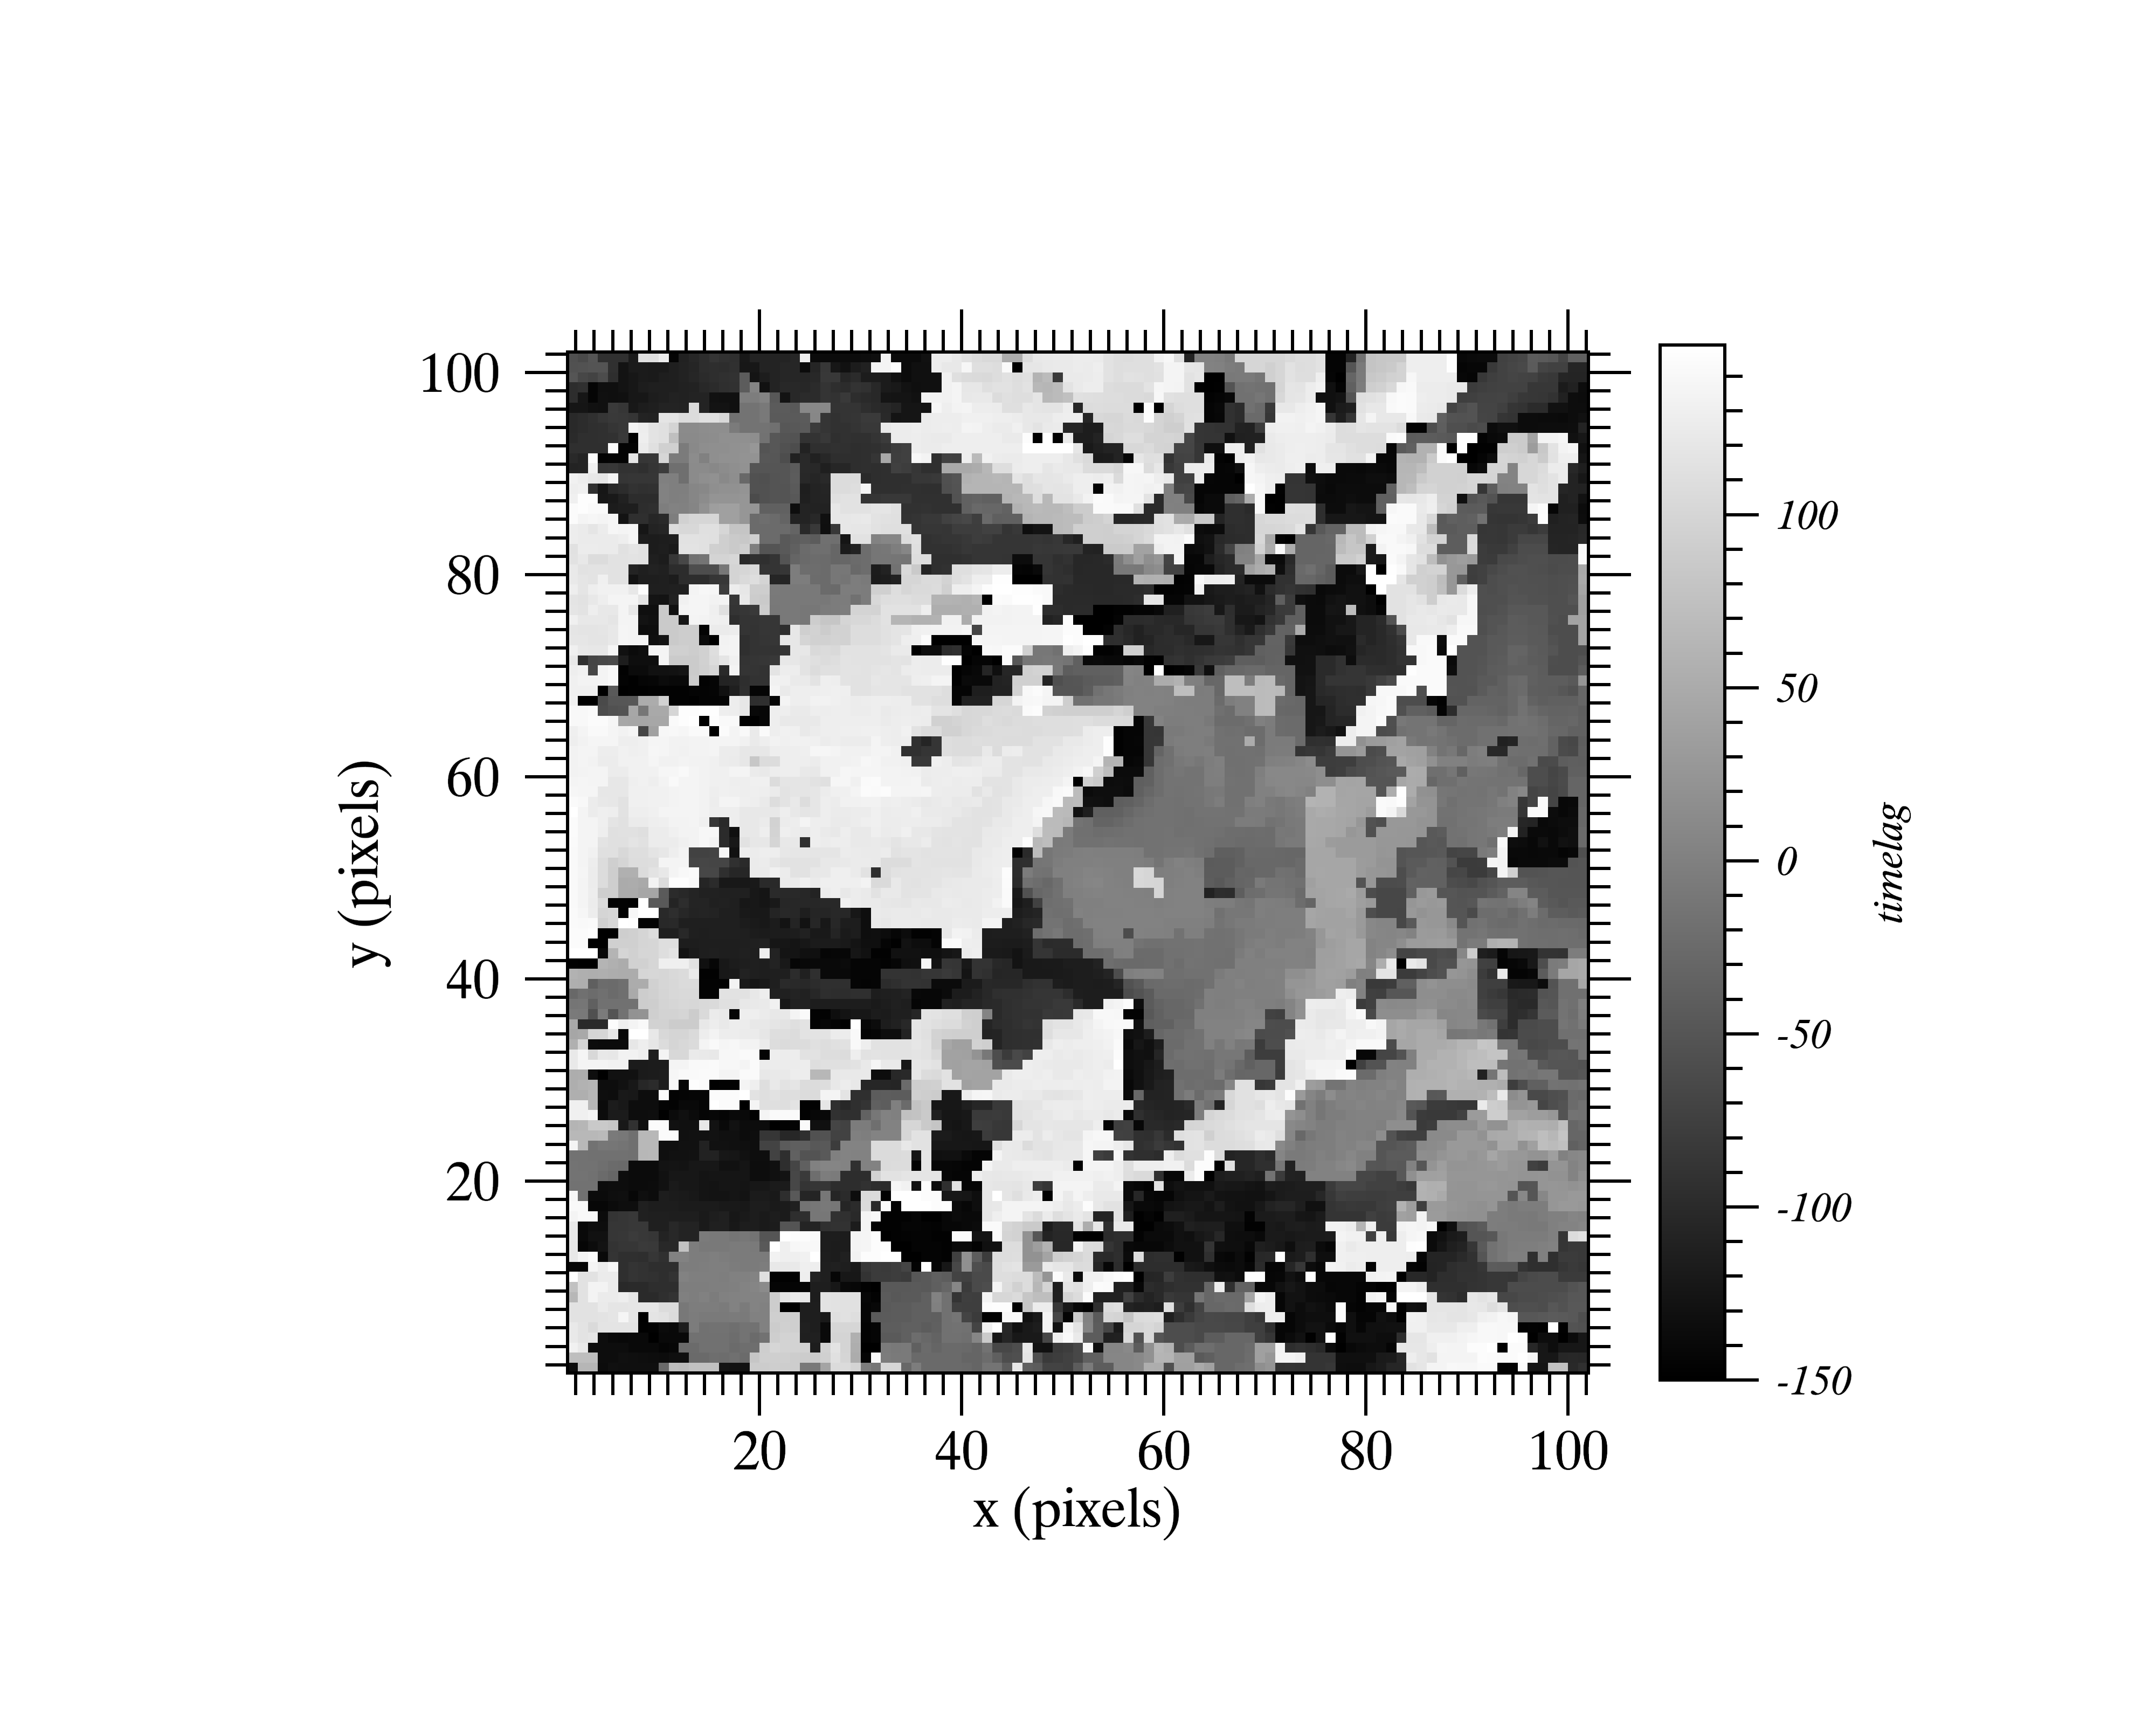
\includegraphics[width=\textwidth]{../figures/bp1_tt.png}
        \caption{Timelag image}
\end{figure}
\begin{figure}[htb!]
        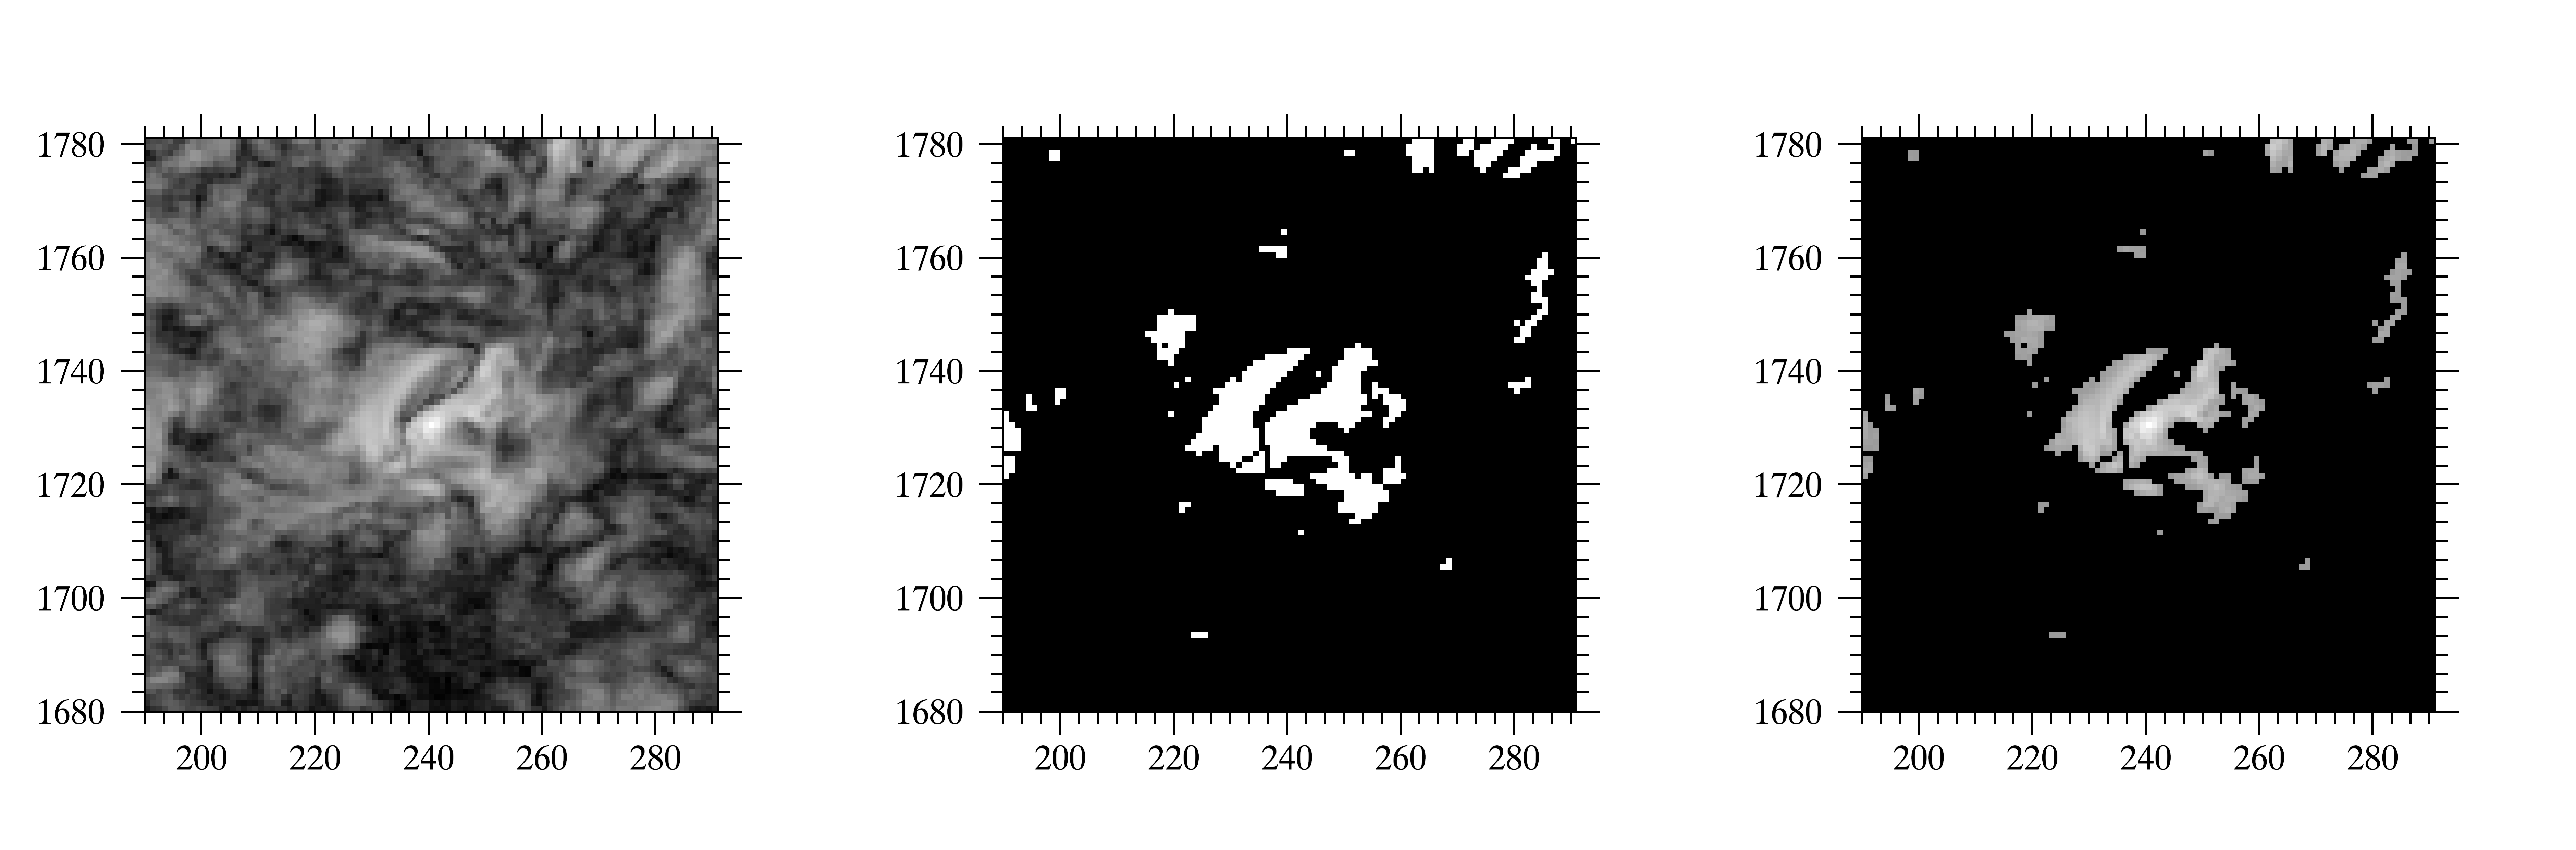
\includegraphics[width=\textwidth]{../figures/bp1_ccMask.png}
        \caption{Left: cross-correlation image of the BP;
        middle: ``mask'' with each cross-correlation pixel greater than
        the threshold (0.6) set equal to 1, and the rest set equal to 0;
        right: multiplication of the first two.}
        \label{ccMask}
\end{figure}
\begin{figure}[h!]
        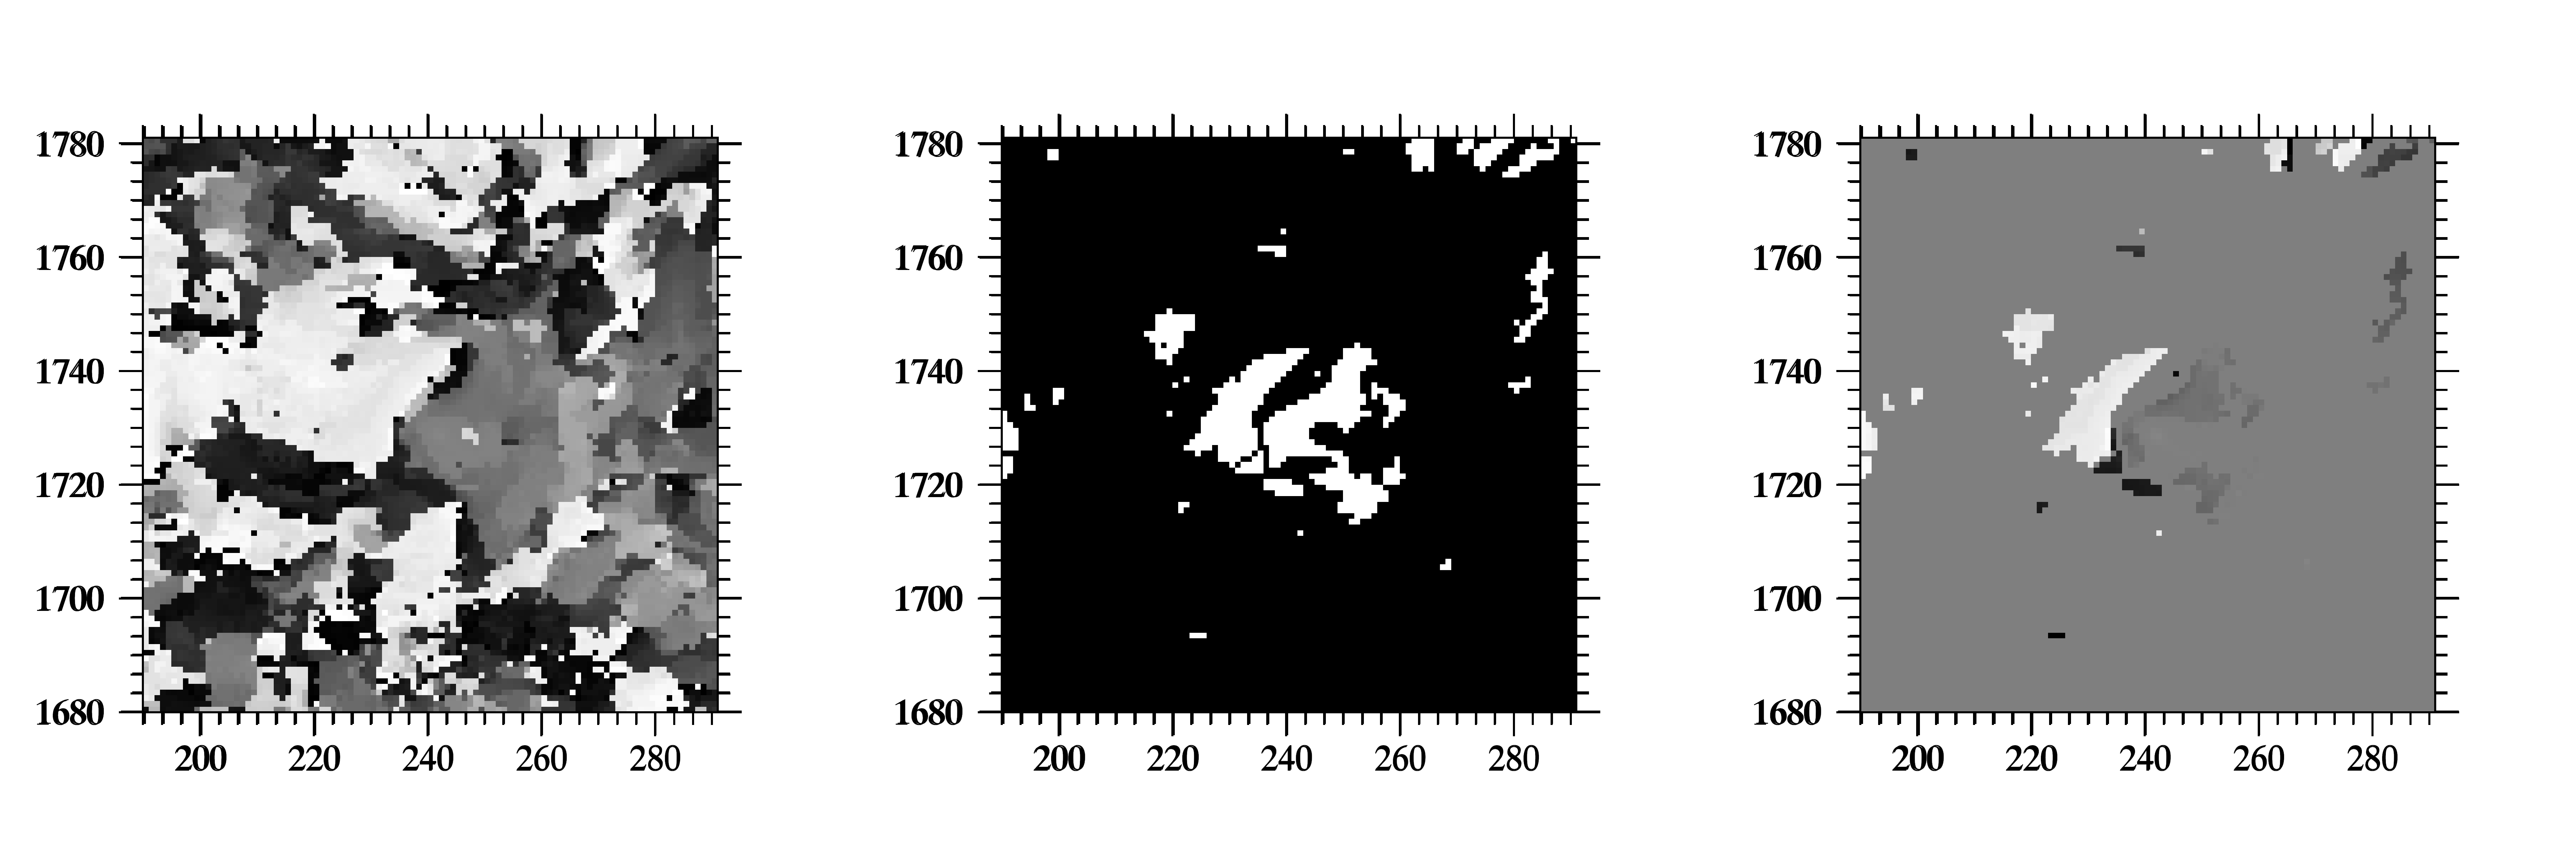
\includegraphics[width=\textwidth]{../figures/bp1_ttMask.png}
        \caption{Left: timelag image of the BP, showing the time
            (still in ``cadence'' units, where each unit is 12 seconds
            apart);
            middle: same mask as in Fig.~\ref{ccMask};
            right: multiplication of the first two.}
\end{figure}

%-------------------------------------------------------------------%

Also plotted are the timelag values at which the
high correlation values occurred, in the next figure, for a pair
of pixel: the one centered at the bright point and another one which
was chosen for a very good reason I'm sure.
The farther the point is, the longer it takes for the motion to
propagate to that point, and therefore the highest cross-correlation
value takes place at a higher timelag value.

The previous figures are ambiguous in direction; it is possible that
features can be evident by propagating in a particular direction, not
necessarily uniformly from the central pixel.

The idea here was to search for distance and timescales that high
cc values occur. The distance will reveal the extent of this structure,
and the timelag will reveal the timescales at which these structures
last.

Why does intensity reveal anything about a possible mesogranular
structure? Or any structure for that matter?
Supergranules exist with diameters of about 30,000 km and last for
roughly two days. Granules have diameters of about 1,000 km and last
for about 12--20 minutes. With only an hour of data, we wouldn't be able
to find anything beyond granule size, unless the timelag values don't
actually correspond to the timescales that these structures last.
Flux tubes in the photosphere are passively moved around until they
eventually fall into the intergranular lanes between supergranules,
where they appear as bright points: low density regions with reduced
opacity where the hotter, brighter interior of the sun becomes visible.

For mesogranulation, we expect a timelag of about 3--5 minutes.
\textcolor{red}{WHY?}

%-------------------------------------------------------------------%

\section{Analysis}


\section{Conclusions}

\bibliography{reffile}
\end{document}

